\documentclass{beamer}
\usepackage[utf8]{inputenc}
\usepackage[T1]{fontenc}
\usepackage{tikz}
\usetikzlibrary{shapes.geometric}
\usepackage{standalone}
\usepackage{amsmath}
\usepackage{amsfonts}
\usepackage{graphicx, color}
\usepackage{svg}

\newcommand{\E}{\mathbb{E}}
\newcommand{\Norm}{\mathcal{N}}
\newcommand{\Loss}{\mathcal{L}}
\newcommand{\R}{\mathbb{R}}
\newcommand{\bt}{\mathbf{t}}
\newcommand{\bU}{\mathbb{U}}
\newcommand{\bu}{\mathbf{u}}
\newcommand{\bw}{\mathbf{w}}
\newcommand{\bX}{\mathbf{X}}
\newcommand{\bx}{\mathbf{x}}
\newcommand{\by}{\mathbf{y}}
\newcommand{\bZ}{\mathbf{Z}}
\newcommand{\bz}{\mathbf{z}}

\newcommand{\eq}{=}
\newcommand{\parfrac}[2]{\frac{\partial #1}{\partial#2}}

\title{Causal Effect Inference with Normalising Flows}
\author{Micha de Groot}


\begin{document}
	
	\begin{frame}
		\titlepage
	\end{frame}
	
	
	\begin{frame}{What is causal inference?} 
		\begin{figure}
            \centering
            \includestandalone{Figures/causal_graph_one_proxy_one_confounder}
            \caption{Causal graph with a latent confounder and observed proxy variable}
            \label{fig:graph_observed_confounder_and_latent_with_proxy}
        \end{figure}
        $$ITE:=\E[\by|\bx, do(\bt=1)] - \E[\by|\bx, do(\bt=0)]$$
	\end{frame}
	
	\begin{frame}{Variational inference and CEVAE}
		$$p(x) \geq \mathcal{L} = \E_{\bz \sim q(\bz|\bx)}[\ln p(\bx|\bz)] - D_{KL}[q(\bz|\bx) || p(\bz)]$$
	\end{frame}
	
	\begin{frame}{Variational inference and CEVAE}
		$$p(x) \geq \mathcal{L} = \E_{\bz \sim q(\bz|\bx)}[\ln p(\bx|\bz)] - D_{KL}[q(\bz|\bx) || p(\bz)]$$
		$$ \mathcal{L} = \E_{\bz \sim q(\bz|\bx)}[\ln p(\bx, \bt, \by|\bz)] - D_{KL}[q(\bz|\bx, \bt, \by) || p(\bz)]$$
	\end{frame}
	
	\begin{frame}{Variational inference and CEVAE}
		$$p(x) \geq \mathcal{L} = \E_{\bz \sim q(\bz|\bx)}[\ln p(\bx|\bz)] - D_{KL}[q(\bz|\bx) || p(\bz)]$$
		$$ \mathcal{L} = \E_{\bz \sim q(\bz|\bx)}[\ln p(\bx, \bt, \by|\bz)] - D_{KL}[q(\bz|\bx, \bt, \by) || p(\bz)]$$
		$$ \mathcal{L} = \E_{\bz \sim q(\bz|\bx)}[\ln p(\bx|\bz) + \ln p(\bt|\bz) + \ln p(\by|\bt, \bz)] - D_{KL}[q(\bz|\bx, \bt, \by) || p(\bz)]$$
	\end{frame}
	
	\begin{frame}{Normalising Flows}
	    Change of variable formula:
	    $$q(\bz') = q(\bz)\left| \det \parfrac{f^{-1}}{\bz'} \right| = q(\bz)\left| \det \parfrac{f}{\bz} \right| ^{-1}$$
	    
	\end{frame}
	
	\begin{frame}{Normalising Flows}
	    $$q(\bz') = q(\bz)\left| \det \parfrac{f^{-1}}{\bz'} \right| = q(\bz)\left| \det \parfrac{f}{\bz} \right| ^{-1}$$
	    $$\bz_K = f_K  \circ ... f_1(\bz_0)$$
	\end{frame}
	
	\begin{frame}{Normalising Flows}
	    $$q(\bz') = q(\bz)\left| \det \parfrac{f^{-1}}{\bz'} \right| = q(\bz)\left| \det \parfrac{f}{\bz} \right| ^{-1}$$
	    $$\bz_K = f_K  \circ ... \circ f_1(\bz_0)$$
	    $$\ln q_K(\bz_K) = \ln q_0(\bz_0) - \sum\limits^K_{k=1} \ln \left|\det \parfrac{f_k}{\bz_{k-1}} \right| $$ 
	\end{frame}
	
	\begin{frame}{Normalising flow: new ELBO}
	     $$\mathcal{L}_{old} = \E_{\bz \sim q(\bz|\bx)}[\ln p(\bx|\bz)] - D_{KL}[q(\bz|\bx) || p(\bz)]$$
	     $$\mathcal{L}_{new} = \E_{\bz_0 \sim q_0(\bz_0)}[\ln p(\bx| \bz_K) + \ln p(\bz_K) - \ln q(\bz_0) + \sum\limits^K_{k=1}\ln \left|\det \parfrac{f_k}{\bz_{k-1}} \right|]  $$
	\end{frame}
	\begin{frame}{Causal inference with Normalising Flows}
	    \centering
	    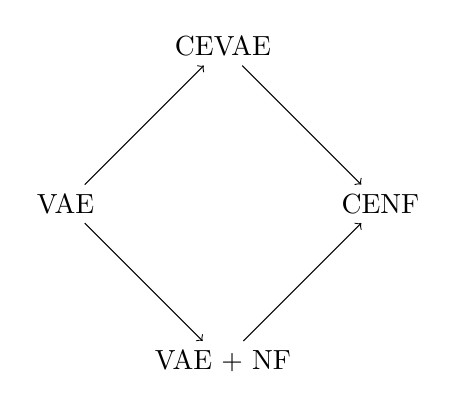
\begin{tikzpicture}
	    \node[] at (0, 0) (VAE) {VAE};
	    \node[] at (2, 2) (CEVAE) {CEVAE};
	    \node[] at (2, -2) (NF) {VAE + NF};
	    \node[] at (4, 0) (CENF) {CENF};
	    
	    \draw[->] (VAE) -- (CEVAE);
	    \draw[->] (VAE) -- (NF);
	    \draw[->] (CEVAE) -- (CENF);
	    \draw[->] (NF) -- (CENF);
	    
	    \end{tikzpicture}
	\end{frame}
	
	\begin{frame}{Causal inference with Normalising Flows}
	    CEVAE:
	    $$ \mathcal{L} = \E_{\bz \sim q(\bz|\bx)}[\ln p(\bx, \bt, \by|\bz)] - D_{KL}[q(\bz|\bx, \bt, \by) || p(\bz)]$$
	    VAE+NF
	    $$\mathcal{L} = \E_{\bz_0 \sim q_0(\bz_0)}[\ln p(\bx| \bz_K) + \ln p(\bz_K) - \ln q(\bz_0) + \sum\limits^K_{k=1}\ln \left|\det \parfrac{f_k}{\bz_{k-1}} \right|]  $$
	\end{frame}
	
	\begin{frame}{Causal inference with Normalising Flows}
	    \begin{equation}\begin{split}
	    \mathcal{L} &= \mathbb{E}_{q_0(\bz_0)}\left[\ln p(\bx, \bt | \bz_K) + \ln p(\bz_K) + \ln p(\by |\bt, \bz_K) - \ln q_0(\bz_0)\right.\\
	    &\left. + \sum\limits^K_{k=1} \ln \left| \det \parfrac{f_k}{\bz_{k-1}}\right| \right]
	    \end{split}\end{equation}
	\end{frame}

    \begin{frame}{Preliminary results}
        \begin{figure}
            \centering
            \includegraphics[scale=0.2]{latex/Figures/Results/metrics_ite.png}
            \caption{Individual Treatment Effect, root of mean square error}
            \label{fig:my_label}
        \end{figure}
    \end{frame}	 
\end{document}